\documentclass[12pt, a4paper, oneside]{report}

% for drawing trees 
\usepackage[linguistics, external]{forest}
\forestset{sn edges/.style={for tree={parent anchor=south, child anchor=north, s sep=10mm, inner sep=0mm}}}
 
\usepackage{tikz}
\usepackage{tikz-qtree}
\tikzset{every tree node/.style={align=center, anchor=north}}
\usetikzlibrary{positioning}

% externalizing figures, helps with compiling
\usetikzlibrary{external}
\tikzexternalize[prefix=tikzz/]

% 
\usepackage{sbe_ma}

\newcommand{\authname}{Name Surname} 
\newcommand{\ttitle}{This is Only a Dummy Thesis Title, Not a Real One \\
Capitalize Your Own Title in the Same Way}
\newcommand{\ttitletr}{Türkçe Tez Başlığı}
\newcommand{\univname}{Boğaziçi University}
\newcommand{\degname}{Master of Arts}
\newcommand{\deptname}{Linguistics}
\newcommand{\supname}{Prof.}
\newcommand{\juryfname}{Prof.}
\newcommand{\jurysname}{Prof.}
%repeat the same in capitals
\newcommand{\authnamecaps}{NAME SURNAME} 
\newcommand{\ttitlecaps}{THESIS TITLE}
\newcommand{\ttitletrcaps}{TÜRKÇE TEZ BAŞLIĞI}
\newcommand{\univnamecaps}{BOĞAZİÇİ UNIVERSITY}
\newcommand{\degnamecaps}{MASTER OF ARTS}
\newcommand{\deptnamecaps}{DEPARTMENT}

\begin{document}

% frontmatter
\pagenumbering{gobble}
% cover page
${}$

\vspace{80pt}

\begin{center}
  \ttitlecaps
\end{center}

\vspace{150pt}

\begin{center}
	\authnamecaps
\end{center}

\vspace{150pt}

\begin{center}
	{\univnamecaps}
\\
  \the\year
\end{center}

\vspace{80pt}
${}$
\newpage
% title page
${}$
\vspace{55pt}


\begin{center}
  \ttitlecaps
\end{center}

\vspace{50pt}

\begin{center}
	Thesis submitted to the\\
	Institute for Graduate Studies in Social Sciences\\
	in partial fulfillment of the requirements for the degree of\\
\end{center}

\vspace{30pt}

\begin{center}
	\degname\\
	in\\
	\deptname
\end{center}

\vspace{30pt}

\begin{center}
	by\\
	\authname
\end{center}

\vspace{30pt}

\begin{center}
  \univname\\
  \the\year
\end{center}

\newpage

\vspace*{2cm}
\begin{center}
 \ttitle
\end{center}

\vspace{2cm}
\begin{center}
  The thesis of \authname\\
  has been approved by:
\end{center}

\vspace*{3cm}

\begingroup
\renewcommand{\arraystretch}{0.5}
\noindent
\begin{tabular}{lp{0.5\textwidth}}
  \supname & \makebox[6.5cm]{\hrulefill}\\
  (Thesis Advisor)&\\
  \vspace*{2em}&\\
  \juryfname & \makebox[6.5cm]{\hrulefill}\\
  \vspace*{3em}&\\
  \jurysname & \makebox[6.5cm]{\hrulefill}\\
  (External Member)&\\
\end{tabular}
\endgroup

\vspace*{\fill}

\begin{center}
	June \the\year
\end{center}

\vspace*{3cm}


\chapter*{\MakeUppercase{declaration of originality}}

\vspace*{20pt}

\noindent I, \authname, certify that 
\begin{itemize} 
	\item I am the sole author of this thesis and that I have fully acknowledged and documented in my thesis all sources of ideas and words, including digital resources, which have been produced or published by another person or institution;
	\item this thesis contains no material that has been submitted or accepted for a degree or diploma in any other educational institution;
	\item this is a true copy of the thesis approved by my advisor and thesis committee at \univname, including final revisions required by them.
\end{itemize}
 
\vspace{40pt}

\noindent Signature: \ldots\ldots\ldots\ldots\ldots.
 
\noindent Date: \ldots\ldots\ldots\ldots\ldots\ldots\dots




\newpage
\pagenumbering{roman}
\setcounter{page}{4}

\chapter*{ABSTRACT\\ \ttitle}
\pagenumbering{roman}
\setcounter{page}{4}

The abstract should consist of a brief, comprehensive summary of the contents of
the thesis. The aim is to allow readers to survey the contents of the thesis
quickly. It should mention the aim of your research, what you did and how you
did it, and the results. It should also indicate the importance of the thesis—what
makes it worth reading, or what it contributes to your field of study. Abstract
length for the Boğaziçi University Institute for Graduate Studies in the Social
Sciences is 250 words maximum, so the abstract should fit onto a single page.
The name of the author does not appear on the abstract page. The Turkish
version of the abstract (with the heading Özet) should reflect the content and
approximate length of the English abstract. As shown above, the word “Abstract”
is capitalized and centered above the title of the thesis. The text of the abstract
itself is double-spaced. Note that the first line is not indented, but begins flush
with the left margin. Normally, an abstract should be a single paragraph. If a
second paragraph is essential, please indent the second paragraph, maintaining
double spacing throughout. 


\newpage

\chapter*{ÖZET\\ \ttitletr}

Bütün insanlar hür, haysiyet ve haklar bakımından eşit doğarlar. Akıl ve vicdana sahiptirler ve birbirlerine karşı kardeşlik zihniyeti ile hareket etmelidirler. Herkes, ırk, renk, cinsiyet, dil, din, siyasi veya diğer herhangi bir akide, milli veya içtimai menşe, servet, doğuş veya herhangi diğer bir fark gözetilmeksizin işbu Beyannamede ilan olunan tekmil haklardan ve bütün hürriyetlerden istifade edebilir. Bundan başka, bağımsız memleket uyruğu olsun, vesayet altında bulunan, gayri muhtar veya sair bir egemenlik kayıtlamasına tabi ülke uyruğu olsun, bir şahıs hakkında, uyruğu bulunduğu memleket veya ülkenin siyasi, hukuki veya milletlerarası statüsü bakımından hiçbir ayrılık gözetilmeyecektir. Yaşamak, hürriyet ve kişi emniyeti her ferdin hakkıdır. Hiç kimse kölelik veya kulluk altında bulundurulamaz; kölelik ve köle ticareti her türlü şekliyle yasaktır. Hiç kimse işkenceye, zalimane, gayriinsani, haysiyet kırıcı cezalara veya muamelelere tabi tutulamaz. Herkes her nerede olursa olsun hukuk kişiliğinin tanınması hakkını haizdir. Kanun önünde herkes eşittir ve farksız olarak kanunun eşit korumasından istifade hakkını haizdir. Herkesin işbu Beyannameye aykırı her türlü ayırdedici mualeleye karşı ve böyle bir ayırdedici muamele için yapılacak her türlü kışkırtmaya karşı eşit korunma hakkı vardır \citep{assembly1948universal}. 


\chapter*{\MakeUppercase{acknowledgements}}


Trial acknowledgement

% moved renew commands for some ToC settings out of sty to here
\renewcommand\contentsname{TABLE OF CONTENTS}
\renewcommand\listfigurename{LIST OF FIGURES}
\renewcommand\listtablename{LIST OF TABLES}
\tableofcontents
\begingroup
\renewcommand{\addvspace}[1]{}
\printglossary[title=\MakeUppercase{abbreviations}, style=block, nonumberlist]
\listoftables
\listoffigures
\endgroup
\clearpage


% main body
\pagenumbering{arabic} 

% YOUR CHAPTERS GO HERE
\chapter{\MakeUppercase{THIS IS AN EXAMPLE OF A LONG CHAPTER TITLE THAT EXTENDS BEYOND ONE LINE}}
% make sure to use \MakeUppercase with your chapter names !!!

The chapter title above shows spacing of a title that does not fit on a single line of
text. Keep it all centered. In deciding where to put the line breaks, try to consider
`thought groups', e.g. it would be less suitable to start the second line with `title' —
the words `chapter' and `title' should be kept together because these two words
refer to a single concept.
Notice that the chapter title is, like the rest of the text, double-spaced. After the
chapter title, there are two double-spaces before the text of the chapter begins.

\section{First-level sub-heading example} \label{firssubsection}

Sub-headings are preceded by two double-spaces. There is only the usual (i.e. one)
double-space between the sub-heading and the first line of the text. Note that there
are two spaces following the number (\ref{firssubsection}) and the first level of the sub-heading.

\subsection{Second-level sub-heading example}

The second-level sub-heading, like the first-level ones, are preceded by two double
spaces. Similarly, there is only one double-space between the sub-heading and the
first line of the text. Remember to put two spaces after the number.

\subsubsection{Third-level sub-heading example}

The spacing for the third-level sub-headings, both vertical and horizontal, is identical
to those of the other sub-headings.

\section{Another first-level sub-heading example that is intended to extend beyond one line}



\chapter{\MakeUppercase{data}}
% make sure to use \MakeUppercase with your chapter names !!!
Although the template is in line with SBE's requirements, it is tailored towards the needs of the linguistics students.

\section{Linguistic examples}

In linguistics, we present examples from the language in question for reflecting the structure in the sentence. Since a reader is not necessarily proficient in that language, we provide glossaries for making the sentence open to analysis, and less mysterious. One important point of glossing a linguistic example is aligning the words with the glosses. Luckily for us {\LaTeX} hosts a package called `gb4e' that provides a way to automatize the process. We also use the package `leipzig' for consistent glossing in our examples, and also reporting what glossaries mean in the list of `GLOSSES'. For an example of a linguistic example see (\ref{linguisticexample}).

\begin{exe}
    \ex \label{linguisticexample}
    \gll 
    Furkan ev-i bul-du. \\ F[{\Nom}] house-{\Acc} find-{\Pst}[{\Third}.{\Sg}] \\
    \glt `Furkan found the house.'
\end{exe}

The glosses you use in your examples are automatically added to the list of glosses in the frontmatter of your thesis, including the glosses you can define in `glossaries.tex' like {\Aor}.

\subsection{Phonological Rules}

We write phonological rules for certain changes or ways that a phonological process takes place. To represent these rules we can use `phonrule' package. For example to represent k-zero alternation in Turkish we can have the rule provided in (\ref{finaldevoicing}).

\begin{exe}
\ex \label{finaldevoicing} \phonb{\phonfeat{stop \\ back} }{[\textgamma]}{V}{V}
\end{exe}

\section{Linguistic trees}

In linguistics we use `trees' that are representational figures that show hierarchical order of how different levels of structural categories are put together. For the most part of the trees you can use the package `forest'. For example see Figure \ref{fig:linguisticexample} for a representation of (\ref{linguisticexample}).

\begin{figure}[hbt!]
    \centering
    \begin{forest}
        [TP 
            [DP\\\textit{Furkan}_i, name=specT]
            [T' 
                [VoiceP 
                    [\sout{DP}_i, name=specVoi]
                    [Voice' 
                        [VP 
                            [DP\\\textit{ev-i}]
                            [V\\\textit{bul}]]
                        [Voice]]]
                [T\\\textit{-du}]]]
    \draw[semithick, dashed, ->] (specVoi) to[out=north west, in=south] (specT);
    \end{forest}
    \caption{An example syntax tree}
    \label{fig:linguisticexample}
\end{figure}

We can also employ feature matrices with our trees as in Figure \ref{fig:linguisticexample2}.
      
\begin{figure}[hbt!]
    \centering
    \begin{forest}
        [TP 
            [\begin{avm}
            \[
                per & {\Third} \\ 
                num & {\Sg} \\
                case & {\Nom} \]
            \end{avm}, name=specT]
            [T' 
                [VoiceP 
                    [\sout{DP}_i, name=specVoi]
                    [Voice' 
                        [VP 
                            [DP\\\textit{ev-i}]
                            [V\\\textit{bul}]]
                        [Voice]]]
                [T\\\textit{-du}]]]
    \draw[semithick, dashed, ->] (specVoi) to[out=west, in=south] (specT);
    \end{forest}
    \caption{Another example syntax tree}
    \label{fig:linguisticexample2}
\end{figure}

If you happen to have any difficulties with drawing trees consult package documentations for `tikz', `tikz-qtree', `forest', and `avm'. This template lets you use all of them in your trees.

\subsection{Additional trees}

\begin{figure}[hbt!]
    \centering
    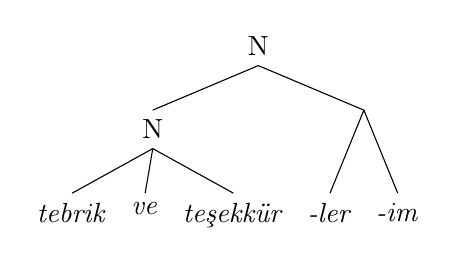
\begin{tikzpicture}
    \Tree[.N
            [.N 
                [.\textit{tebrik} ]
                [.\textit{ve} ]
                [.\textit{teşekkür} ] ]
            [ 
                [.\textit{-ler} ]
                [.\textit{-im} ] ]
    ];
    \end{tikzpicture}
    \caption{{\Pl} and {\Poss} forming a complex head in grammatical SA}
    \label{fig:furkan2}
\end{figure}

All human beings are born free and equal in dignity and rights. They are endowed with reason and conscience and should act towards one another in a spirit of brotherhood. Everyone is entitled to all the rights and freedoms set forth in this Declaration, without distinction of any kind, such as race, colour, sex, language, religion, political or other opinion, national or social origin, property, birth or other status. Furthermore, no distinction shall be made on the basis of the political, jurisdictional or international status of the country or territory to which a person belongs, whether it be independent, trust, non-self-governing or under any other limitation of sovereignty. Everyone has the right to life, liberty and security of person. No one shall be held in slavery or servitude; slavery and the slave trade shall be prohibited in all their forms. No one shall be subjected to torture or to cruel, inhuman or degrading treatment or punishment. Everyone has the right to recognition everywhere as a person before the law. All are equal before the law and are entitled without any discrimination to equal protection of the law. All are entitled to equal protection against any discrimination in violation of this Declaration and against any incitement to such discrimination.
\begin{figure}[hbt!]
    \centering
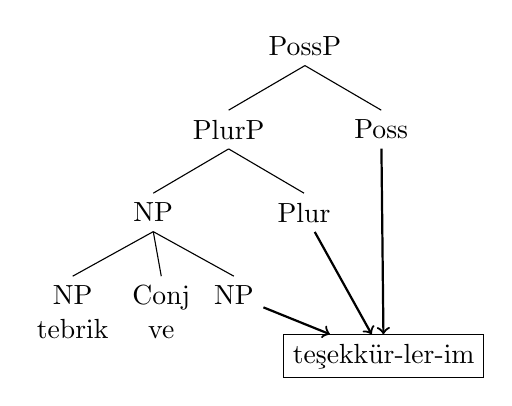
\begin{tikzpicture}
    \Tree[.PossP
            [.PlurP 
                [.NP 
                    [.NP\\tebrik ]
                    [.Conj\\ve ]
                    [.\node(NP2){NP}; ] ]
                [.\node(plr){Plur}; ] ]
            [.\node(PS){Poss}; ]
]
\node[below right= 1em of NP2, draw](co){teşekkür-ler-im};
\draw[thick, ->] (NP2) -- (co);
\draw[thick, ->] (plr) -- (co);
\draw[thick, ->] (PS) -- (co);
\end{tikzpicture}
    \caption{Lexical sharing analysis of {\Pl} and {\Poss} in SA}
    \label{fig:lexicalshare}
\end{figure}

All human beings are born free and equal in dignity and rights. They are endowed with reason and conscience and should act towards one another in a spirit of brotherhood. Everyone is entitled to all the rights and freedoms set forth in this Declaration, without distinction of any kind, such as race, colour, sex, language, religion, political or other opinion, national or social origin, property, birth or other status. Furthermore, no distinction shall be made on the basis of the political, jurisdictional or international status of the country or territory to which a person belongs, whether it be independent, trust, non-self-governing or under any other limitation of sovereignty. Everyone has the right to life, liberty and security of person. No one shall be held in slavery or servitude; slavery and the slave trade shall be prohibited in all their forms. No one shall be subjected to torture or to cruel, inhuman or degrading treatment or punishment. Everyone has the right to recognition everywhere as a person before the law. All are equal before the law and are entitled without any discrimination to equal protection of the law. All are entitled to equal protection against any discrimination in violation of this Declaration and against any incitement to such discrimination.
\begin{figure}[hbt!]
    \centering
    \begin{forest}
        [ConjP, s sep=30mm 
            [Conj' 
                [TP 
                    [DP\\\textit{Ahmet}_i]
                    [T'
                        [VoiceP 
                            [\sout{DP}_i]
                            [Voice' 
                                [VP 
                                    [\sout{DP}, name=tk]
                                    [V\\\textit{al}]]
                                [Voice]]]
                        [T\\\textit{-dı}]]]
                [Conj\\\textit{ve}]
                [TP 
                    [DP\\\textit{Mehmet}_j]
                    [T' 
                        [VoiceP 
                            [\sout{DP}_j] 
                            [Voice' 
                                [VP 
                                    [\sout{DP}, name=tl]
                                    [V\\\textit{sat}]]
                                [Voice]]]
                        [T\\\textit{-tı}]]]]
            [DP\\\textit{kitab-ı}, name=DP ]]
        \draw[rounded corners=1em, ->] (tk.south) -- ++(south:2.5em) -| (DP.south);
        \draw[rounded corners=1em, ->] (tl.south) -- ++(south:1.5em) -| (DP.south);
    \end{forest}
    \caption{RNR analysis for Backward Ellipsis}
    \label{fig:backwardellipsis}
\end{figure}



\section{Linguistic tables}

The normal tabularx environments are enough for generic table uses. However a linguistics student might need to use an Optimality Theory tableau in representing (mostly) phonological processes. For special characters that are used in IPA (international phonetic alphabet), we use the package `tipa' consult package documentation for more information. Now we can try to form a tableau for k-zero alternation in a Turkish expression like `\textit{öğren-me/k/-i}' learn-{\Inf}-{\Acc}, where there is free variation among people between \phon{/k/}{[\textgamma]} and \phon{k}{[j]}. See Table \ref{tab:kzero} for an OT tableau.

\begin{table}[hbt!]
    \caption{OT Tableau for k-zero Alternation}
    \vspace{10pt}
    \centering
    \begin{tableau}{c:c|c}
        \inp{\ips{\oe :\textfishhookr\textepsilon nm\textepsilon k}} \const{*STOP} \const{PALATAL}
        \cand{\oe :\textfishhookr\textepsilon nm\textepsilon k} \vio{*!} \vio{}
        \cand{\oe :\textfishhookr\textepsilon nm\textepsilon\textgamma} \vio{} \vio{*}
        \cand[\Optimal]{\oe :\textfishhookr\textepsilon nm\textepsilon j} \vio{} \vio{}
    \end{tableau}

    \label{tab:kzero}
\end{table}

Please remember that SBE follows a different Table and Figure caption placement. As of this template is being formed Table captions come above the Tables and Figure captions come below the Figure environments. Be sure to check SBE's editor guidelines for up to date information. All of the Figures and Tables are automatically added to the list of tables and list of figures with their caption name and the number of the page they appear in, with the SBE required stylistic customizations. An example for in-text citing where \cite{atmaca2020} talks about making an MA template complying with SBE guidelines \citep{atmaca2020} is just given.



\section{Why {\LaTeX}?}

Some of the advantages that {\LaTeX} provides include:

\begin{itemize}
    \item Presenting linguistic examples consistently
    \item Representing the data with tailored figures 
    \item Only the references used in-text are listed at the end automatically
    \item Cross-referencing linguistic examples, figures, and tables 
\end{itemize}

\section{Additional tables}
All human beings are born free and equal in dignity and rights. They are endowed with reason and conscience and should act towards one another in a spirit of brotherhood. Everyone is entitled to all the rights and freedoms set forth in this Declaration, without distinction of any kind, such as race, colour, sex, language, religion, political or other opinion, national or social origin, property, birth or other status. Furthermore, no distinction shall be made on the basis of the political, jurisdictional or international status of the country or territory to which a person belongs, whether it be independent, trust, non-self-governing or under any other limitation of sovereignty. Everyone has the right to life, liberty and security of person. No one shall be held in slavery or servitude; slavery and the slave trade shall be prohibited in all their forms. No one shall be subjected to torture or to cruel, inhuman or degrading treatment or punishment. Everyone has the right to recognition everywhere as a person before the law. All are equal before the law and are entitled without any discrimination to equal protection of the law. All are entitled to equal protection against any discrimination in violation of this Declaration and against any incitement to such discrimination.

\begin{table}[hbt!]
\caption{Verbal Terminal Morphemes}
\vspace{10pt}
    \centering
    \begin{tabular}{|ll|}
    \hline 
                                    {(i) Agreement markers} &  \\ \hline
                                    \multirow{5}{20em}{(ii) Aspect/ Modality markers}  & {\Aor} \textit{-(I)r/(A)r} \\ 
                                                            & {\Prog} \textit{-Iyor} \\
                                                            & {\Fut} \textit{-(y)AcAK} \\
                                                            & {\Evi} \textit{-mIş} \\
                                                            & {\Nec} \textit{-mAlI} \\ \hline
        \multirow{2}{20em}{(iii) Converb markers}           & \textit{-(y)IncA} \\
                                                            & \textit{-(y)Ip} \\
    \hline                                                         
    \end{tabular}
    \label{tab:terminalmorphemes}
\begin{flushright}
    Adapted from \cite{kabak2007turkish}
\end{flushright}
\end{table}

All human beings are born free and equal in dignity and rights. They are endowed with reason and conscience and should act towards one another in a spirit of brotherhood. Everyone is entitled to all the rights and freedoms set forth in this Declaration, without distinction of any kind, such as race, colour, sex, language, religion, political or other opinion, national or social origin, property, birth or other status. Furthermore, no distinction shall be made on the basis of the political, jurisdictional or international status of the country or territory to which a person belongs, whether it be independent, trust, non-self-governing or under any other limitation of sovereignty. Everyone has the right to life, liberty and security of person. No one shall be held in slavery or servitude; slavery and the slave trade shall be prohibited in all their forms. No one shall be subjected to torture or to cruel, inhuman or degrading treatment or punishment. Everyone has the right to recognition everywhere as a person before the law. All are equal before the law and are entitled without any discrimination to equal protection of the law. All are entitled to equal protection against any discrimination in violation of this Declaration and against any incitement to such discrimination.
\begin{table}[hbt!]
    \caption{Response of Different Category Suffixes in Korean to Lexical Integrity Tests}
    \vspace{10pt}
    \centering
    \begin{tabular}{|p{1.8cm}|p{2.1cm}|p{1.7cm}|p{1.6cm}|p{1.6cm}|p{2cm}|p{1.8cm}|}
    \hline 
                        & Coordination & External Modifiers & Gapping (Base) & Gapping (Suffix) & Inbound Ana Island & Extraction \\ \hline 
    Opaque Suffix       & N             & N                 & N             & N                 & N   & N \\ \hline 
    Transparent Suffix  & Y             & Y                 & N             & Y                 & Y   & N \\ \hline 
    Double-duty Suffix  & N/Y           & N/Y               & N             & N/Y               & N/Y & N/Y \\ \hline 
    \end{tabular}
    \label{tab:korean}
\end{table}

All human beings are born free and equal in dignity and rights. They are endowed with reason and conscience and should act towards one another in a spirit of brotherhood. Everyone is entitled to all the rights and freedoms set forth in this Declaration, without distinction of any kind, such as race, colour, sex, language, religion, political or other opinion, national or social origin, property, birth or other status. Furthermore, no distinction shall be made on the basis of the political, jurisdictional or international status of the country or territory to which a person belongs, whether it be independent, trust, non-self-governing or under any other limitation of sovereignty. Everyone has the right to life, liberty and security of person. No one shall be held in slavery or servitude; slavery and the slave trade shall be prohibited in all their forms. No one shall be subjected to torture or to cruel, inhuman or degrading treatment or punishment. Everyone has the right to recognition everywhere as a person before the law. All are equal before the law and are entitled without any discrimination to equal protection of the law. All are entitled to equal protection against any discrimination in violation of this Declaration and against any incitement to such discrimination.
\begin{table}[hbt!]
    \caption{Mari Nominal Domain Morpheme Order}
    \vspace{10pt}
    \centering
    \begin{tabular}{|ll|}
    \hline 
        {\Pl} \textgreater {\Poss} & \textit{pasu-vlak-na}  \\
        {\Poss} \textgreater {\Pl} & \textit{pasu-na-vlak} \\ \hline
        {\Pl} \textgreater {\Lcase} & \textit{pasu-vlak-e\u{s}te} \\
        {\Pl} \textgreater {\Scase} & \textit{pasu-vlak-em} \\ \hline
        {\Lcase} \textgreater {\Poss} & \textit{pasu-\u{s}te-na} \\
        {\Poss} \textgreater {\Scase} & \textit{pasu-na-m} \\ \hline
        {\Pl} \textgreater {\Lcase} \textgreater {\Poss} & \textit{pasu-vlak-e\u{s}te-na} \\
        {\Poss} \textgreater {\Pl} \textgreater {\Lcase} & \textit{?pasu-na-vlak-e\u{s}te} \\ \hline
        {\Pl} \textgreater {\Poss} \textgreater {\Scase} & \textit{pasu-vlak-na-m} \\
        {\Poss} \textgreater {\Pl} \textgreater {\Scase} & \textit{pasu-na-vlak-em} \\ \hline 
        \multicolumn{2}{|l|}{\textit{pasu} `garden', \textit{-vlak} {\Pl}, \textit{-na} {\Poss}.{\First}.{\Pl}, \textit{-(e)\u{s}te} {\Iness}, \textit{-(e)m} {\Acc}} \\
        \hline 
    \end{tabular}
    \label{tab:mariorder} \\
    ${}$ \\ \hfill Adapted from \cite{guseva2017postsyntactic}
\end{table}

\begin{table}[hbt!]
    \caption{Feature Geometry of {\Poss} in Turkish}
    \centering
    \begin{tabular}{|l|l|l|}
    \hline
         \multicolumn{2}{|c|}{Features} & \multirow{2}{*}{Exponent}  \\ \cline{1-2}
         Participant & Individuation  & \\ \hline
         Speaker & $\emptyset$ & \textit{-Im} \\ \hline 
         Addressee & $\emptyset$ & \textit{-In} \\ \hline 
         Speaker & Group & \textit{-ImIz} \\ \hline 
         Addressee & Group & \textit{-InIz} \\ \hline 
         $\emptyset$ & $\emptyset$ & \textit{-(s)I(n)} \\ \hline 
         $\emptyset$ & Group & \textit{-lArI} \\ \hline 
    \end{tabular}
    \label{tab:kharyfeatures}
\end{table}


\chapter{\MakeUppercase{experiment}}
% make sure to use \MakeUppercase with your chapter names !!!

\chapter{\MakeUppercase{analysis}}
% make sure to use \MakeUppercase with your chapter names !!!

\chapter{\MakeUppercase{discussion}}
% make sure to use \MakeUppercase with your chapter names !!!

\chapter{\MakeUppercase{conclusion and future work}}
% make sure to use \MakeUppercase with your chapter names !!!



% endmatter
\appendix
% changing chapter heading for table of content
\addtocontents{toc}{\protect\setcounter{tocdepth}{0}}
\titlecontents{chapter}[0pt]{}{\MakeUppercase{appendix \thecontentslabel:\quad}\MakeUppercase}{}{\dotfill\contentspage}


\setlength\RaggedRightParindent{0cm}
% PUT YOUR APPENDICIES HERE BY CALLING INPUT FUNCTION %
\chapter{SAMPLES OF SEMI-STRUCTURED QUESTIONS}

\begin{enumerate}
    \item Could you tell me when you started learning English?
    \item Could you describe a typical school day at your university campus?
    \item Could you tell me about a recent English lesson?
    \item For what sorts of things do you use English outside the classroom?
    \item Can you tell me about a recent speaking event that happened outside the
classroom?
    \item How would you complete this sentence: I know English and …
\end{enumerate}

\doublespacing
\chapter{TRIAL 2}


\setlength\RaggedRightParindent{1.27cm}


\newpage

% for printing references
\singlespacing
\addcontentsline{toc}{chapter}{REFERENCES}
\renewcommand\bibname{REFERENCES}
\begingroup
\raggedright
\setlength\bibhang{0.5in}
\bibliographystyle{spa_ma}
\bibliography{references}
\endgroup
% \wordcount






\end{document}
